\section*{\nr.3 \titthree (25 Punkte)}
\begin{enumerate}[(a)]
\item Unter dem Winkel $\alpha$ gibt es für zwei Wellen, einen Gangunterschied 
\begin{equation}
  \delta = \sin \alpha g
\end{equation}
dies resultiert in einem Phasenunterschied von
\begin{equation}
  \varphi = \frac{2 \pi \delta}{\lambda}=\frac{2 \pi \sin \alpha g}{\lambda}
\end{equation}
\item Es gilt 
\begin{align}
  E=\sum_{n=1}^N\exp\left(i\varphi n\right)&=\frac{\exp\left(i\varphi n\right) -1}{\exp\left(i \varphi\right)-1}
  \\&=\frac{\exp\left(i\varphi N/2\right)}{\exp\left(i \varphi/2\right)}\cdot \left(\frac{\exp\left(i\varphi N/2\right)-\exp\left(-i\varphi N/2\right)}{\exp\left(i\varphi /2\right)-\exp\left(-i\varphi/2\right)}\right)\\
  &=\frac{\exp\left(i\varphi N/2\right)}{\exp\left(i \varphi/2\right)}\cdot \frac{\sin\left(\varphi N/2\right)}{\sin\left(\varphi/2\right)}
\end{align}
Da $|\exp i a| = 1 \forall a$ folgt 
\begin{equation}
  |E|=\frac{\sin\left(N \varphi/2\right)}{\sin\left(\varphi/2\right)}
\end{equation}
und damit
\begin{equation}
  |E|^2=\frac{\sin^2\left(N \varphi/2\right)}{\sin^2\left(\varphi/2\right)}
\end{equation}
\item Die Ergebnisse der Monte-Carlo-Simulation mit dem zur Verfügung gestellten Python-Skript (ein Normierungsfehler wurde korrigiert) sind in \vref{fig:montecarlo} dargestellt.
\begin{figure}[htbp]
\centering
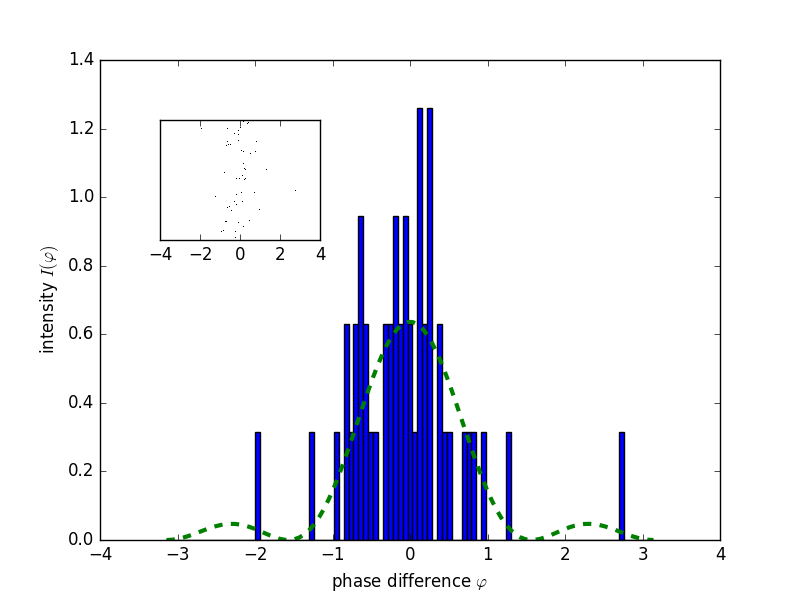
\includegraphics[width=0.49\textwidth]{50.png}
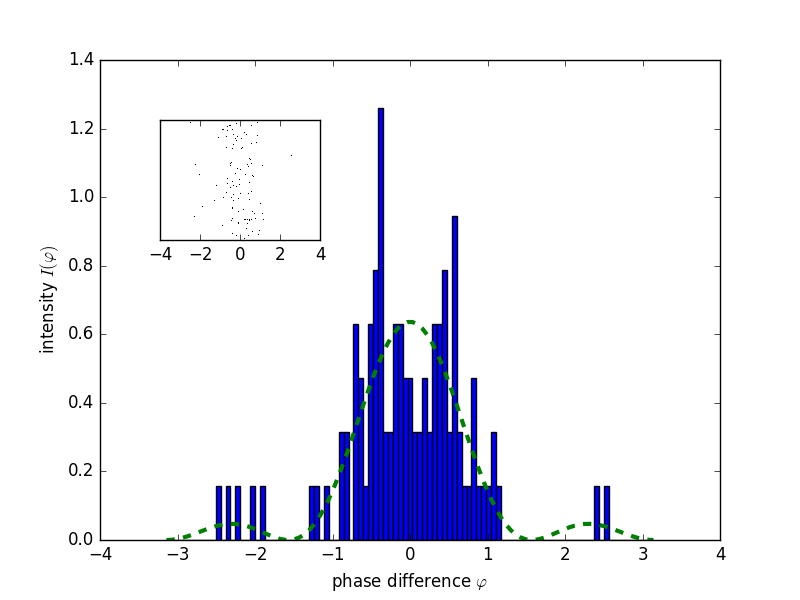
\includegraphics[width=0.49\textwidth]{100.png}
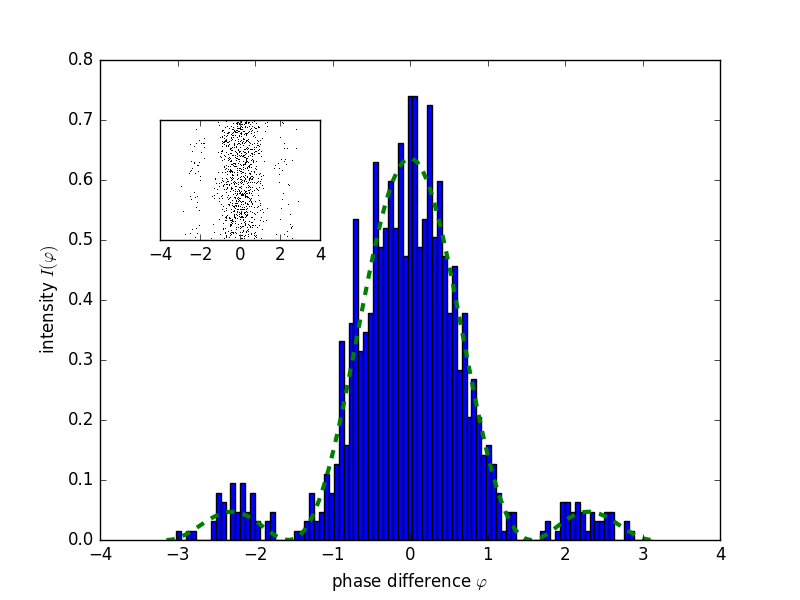
\includegraphics[width=0.49\textwidth]{1000.png}
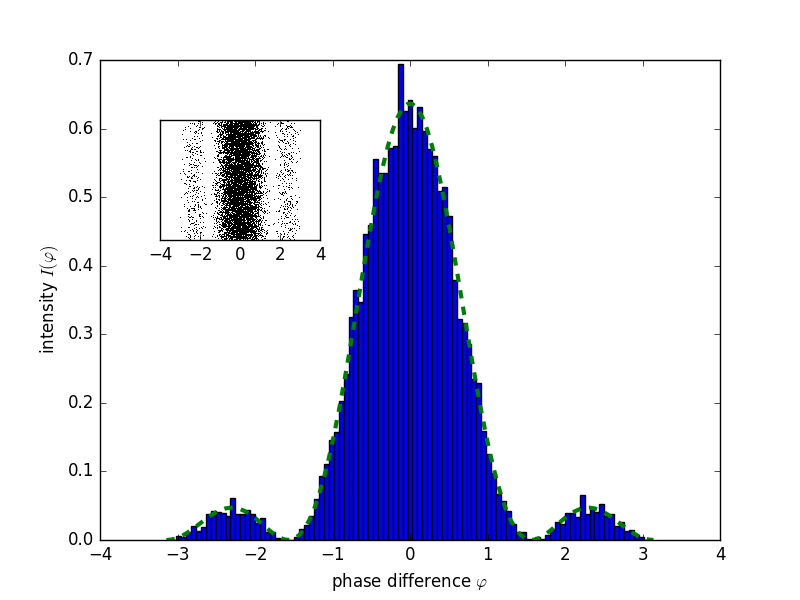
\includegraphics[width=0.49\textwidth]{10000.png}
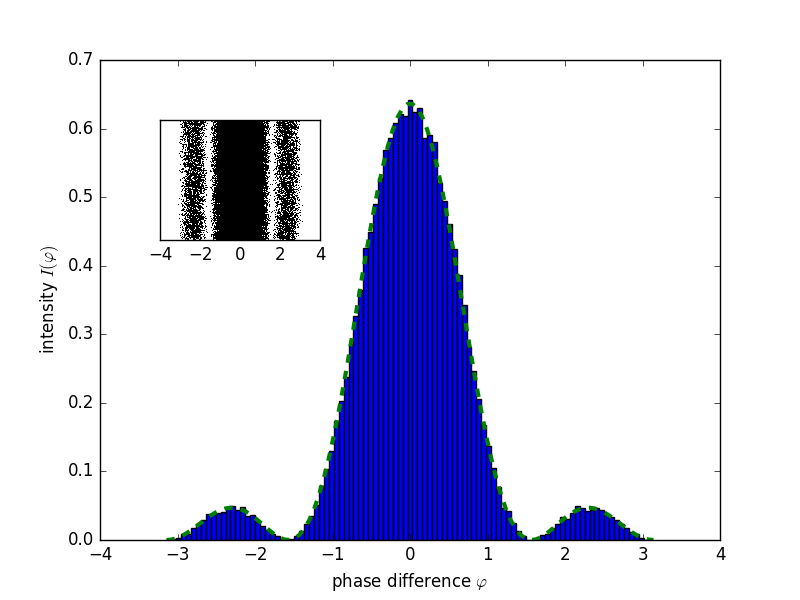
\includegraphics[width=0.49\textwidth]{100000.png}
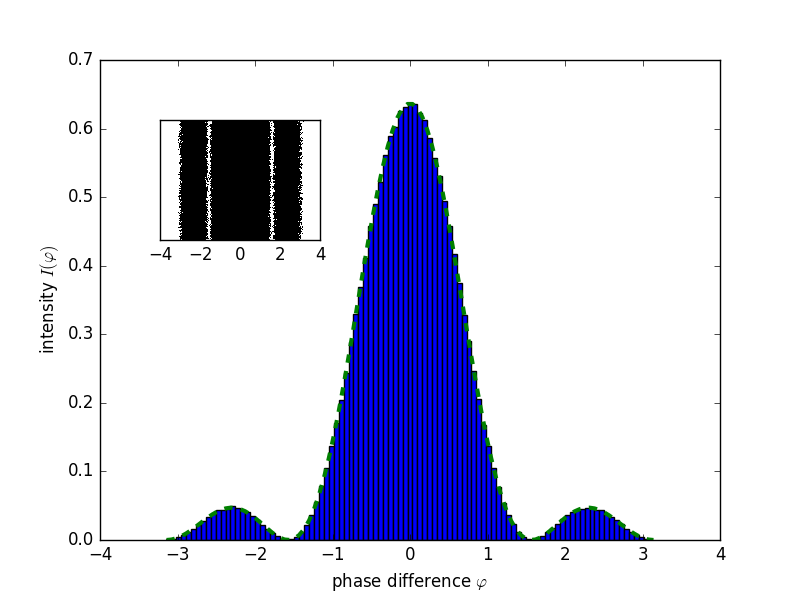
\includegraphics[width=0.49\textwidth]{1000000.png}
\caption{Ergebnisse für verschiedene Anzahl an Versuchen, von links oben nach rechts unten: $n=50,100,1000,10000,100000,1000000$}
\label{fig:montecarlo}
\end{figure}
Ab wann genau das Interferenzmuster erkennbar ist, ist schwer zu sagen und sehr subjektiv. Ab ca. 1000 Durchführungen sind jedoch auch die Nebenmaxima eindeutig erkennbar.
\end{enumerate}
